\documentclass{notes}

\title{A Coherent Presentation Practce}
\author{16423 Yota Toyama}
\date{}


\begin{document}

\maketitle

Hello, everyone.
Today, I would like to introduce my research to you.

My research's theme is sentiment classification of documents
by machine learning.
First, let me explain about the 2 main terms, sentiment classification
and machine learning.
The first one, sentiment classification is a task
in which we classify something into 2 or more classes by its sentiment.
Sentiment is a kind of emotion, feeling or reputation for something.
For example, the number of stars given to the products on Amazon's website
is a sort of sentiment representation.
The second one, machine learning is a way to let computers learn something.
More mathematically, it is a way to find the best function
giving the most appropriate output to each input automatically by algorithm
which is implemented as a computer program.
In fact, while finding the best function from the entire set
of possible functions is a hard problem, we define a model,
one subset of the entire function set, having parameters
and find the best function by optimizing its parameters.
In summary, my research is about how to find the best function,
so called a classifier, which takes a document as input
and the most appropriate sentiment representation for it as output.
And, the purpose of it is proposing a model which can become the best function
by parameter optimization.
Every paper about machine learning usually about a model the authors propose
and describes how good performance the model achived.
\begin{gather*}
  y = f(x; w) \\
  \begin{cases}
    y : \text{Output} \\
    f : \text{A model} \\
    x : \text{Input} \\
    w : \text{Parameters of the model}
  \end{cases}
\end{gather*}
\begin{figure*}
  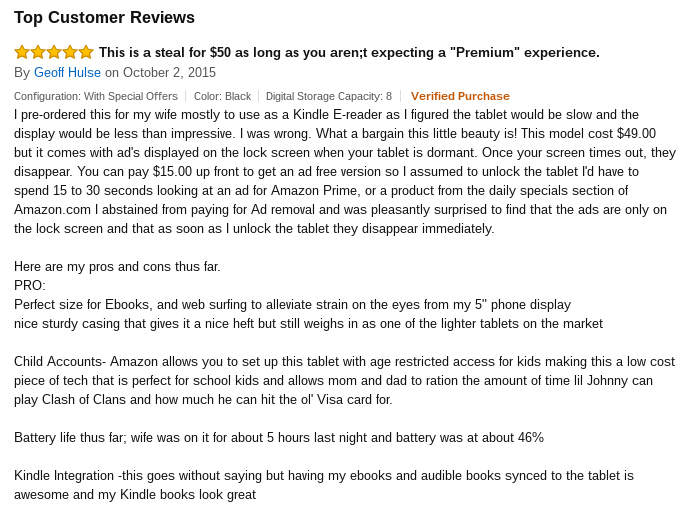
\includegraphics[width=\textwidth]{fig/review.png}
\end{figure*}

As others, our research proposes a new model.
Then, let me show you what is our new model.
The features of our model are as follows.
\begin{enumerate}
  \item The model uses the method of Artificial Neural Network (ANN).
  \item The model takes fonts in the document as input.
  \item The prior knowledge about the document structure
        from characters to documents is incorpolated into the model.
\end{enumerate}
Let me describe the each items.
First, ANN is a model which imitates the mechanism of brains we have.
Aside from the relation of ANN and brains, an ANN model can be represented
as a mathematical matrix function.
Second, probably, fonts have been much familiar to you.
A font is an image corresponding to a specific character
and mainly used in computers to display characters to screens.
Third, the model uses structures of documents as inputs.
As you know, a document is made up of sentences
and a sentence is made up of words and so on.
Summarizing all in the list,
the model classifies documents into sentiment classes
building and representing fonts, characters, words, sentences, a document
and its sentiment as matrices, vectors, or scalars.

\end{document}
